%%%%%%%%%%%%%%%%%%%%%%%%%%%%%%%%%%%%%%%%%%%%%%%%%%%%%%%%%%%%%%%%%%%%%%%%%%%%%%%%%%
\begin{frame}[fragile]\frametitle{}
\begin{center}
{\Large MLOps in Production: The Bigger Picture}
\end{center}
\end{frame}

%%%%%%%%%%%%%%%%%%%%%%%%%%%%%%%%%%%%%%%%%%%%%%%%%%%%%%%%%%
\begin{frame}[fragile]\frametitle{What DevOps Does}
\begin{itemize}
\item DevOps joins software development (Dev) and operations (Ops) through automation
\item Version control: every change is tracked in git
\item Continuous integration (CI): build and test the code on every commit
\item Continuous delivery (CD): release to production automatically and repeatably
\item Infrastructure as code: servers and networks are described in files, not set up by hand
\item Containers and orchestration: the same package runs everywhere
\item Monitoring and logging: watch the running system, alert, and respond to incidents
\end{itemize}
\end{frame}

%%%%%%%%%%%%%%%%%%%%%%%%%%%%%%%%%%%%%%%%%%%%%%%%%%%%%%%%%%
\begin{frame}[fragile]\frametitle{MLOps = DevOps + Data + Models}
MLOps applies DevOps ideas to ML systems, where data and models change as well as code:
\begin{center}
\small\renewcommand{\arraystretch}{1.35}
\begin{tabular}{>{\raggedright\arraybackslash}p{0.3\linewidth}>{\raggedright\arraybackslash}p{0.62\linewidth}}
\hline
\textbf{DevOps} & \textbf{What ML adds} \\
\hline
CI: test the code & also validate the data (schema, value ranges) and the model \\
CD: deploy a service & deploy a whole training pipeline, and the model service it produces \\
(nothing similar) & CT, continuous training: retrain and re-serve models automatically \\
Monitor uptime and errors & also monitor data drift and model quality \\
\hline
\end{tabular}
\end{center}
{\tiny (Ref: Google Cloud, MLOps: Continuous delivery and automation pipelines in machine learning)}
\end{frame}

%%%%%%%%%%%%%%%%%%%%%%%%%%%%%%%%%%%%%%%%%%%%%%%%%%%%%%%%%%
\begin{frame}[fragile]\frametitle{MLOps Maturity Levels}
\begin{center}
\small\renewcommand{\arraystretch}{1.35}
\begin{tabular}{>{\raggedright\arraybackslash}p{0.2\linewidth}>{\raggedright\arraybackslash}p{0.42\linewidth}>{\raggedright\arraybackslash}p{0.28\linewidth}}
\hline
\textbf{Level} & \textbf{What is automated} & \textbf{Retraining trigger} \\
\hline
0: Manual & nothing: notebooks, hand-offs, a few releases a year & a person decides \\
1: Pipeline automation & the training pipeline: modular, containerized, reproducible & schedule, new data, performance drop, drift \\
2: CI/CD automation & the pipeline and its build, test and deployment & as level 1, plus automated release of pipeline changes \\
\hline
\end{tabular}
\end{center}
Most teams start at level 0. Move up when releases become frequent or manual steps cause errors.

{\tiny (Ref: Google Cloud, MLOps: Continuous delivery and automation pipelines in machine learning)}
\end{frame}

%%%%%%%%%%%%%%%%%%%%%%%%%%%%%%%%%%%%%%%%%%%%%%%%%%%%%%%%%%
\begin{frame}[fragile]\frametitle{The Production Loop}
\adjustbox{valign=t}{%
\begin{minipage}{0.5\linewidth}
\begin{itemize}
\item Production ML is a loop, not a line
\item Every arrow can be automated
\item Validate before you register; register before you deploy
\item Monitoring and user feedback flow back into new data
\item New data feeds the next round of training
\end{itemize}
\end{minipage}%
}%
\hfill%
\adjustbox{valign=t}{%
\begin{minipage}{0.46\linewidth}
\begin{center}
\adjustbox{max width=\linewidth, max totalheight=5.5cm}{%
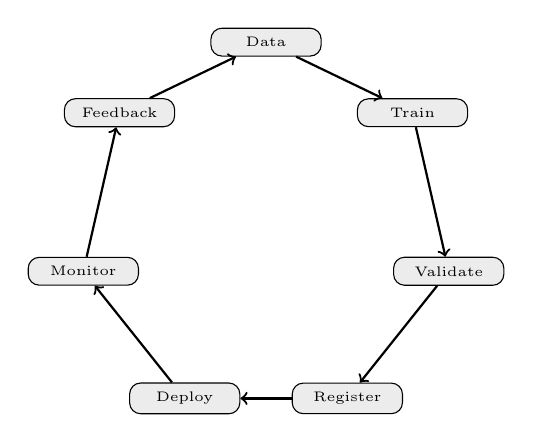
\begin{tikzpicture}[scale=0.7, every node/.style={font=\tiny}]
\foreach \i/\lab in {0/Data,1/Train,2/Validate,3/Register,4/Deploy,5/Monitor,6/Feedback} {
  \node[draw, rounded corners, minimum width=1.4cm, fill=gray!15] (n\i) at ({90-360/7*\i}:3.4) {\lab};
}
\foreach \i/\j in {0/1,1/2,2/3,3/4,4/5,5/6,6/0} { \draw[->, thick] (n\i) -- (n\j); }
\end{tikzpicture}%
}
\end{center}
\tiny{The production loop: feedback closes it.}
\end{minipage}%
}
\end{frame}

%%%%%%%%%%%%%%%%%%%%%%%%%%%%%%%%%%%%%%%%%%%%%%%%%%%%%%%%%%
\begin{frame}[fragile]\frametitle{How Data Is Curated}
\begin{itemize}
\item Collect: log inputs and outcomes from the running system, within privacy rules
\item Validate: check schema, ranges, missing values and duplicates before training (for example with Great Expectations)
\item Clean and label: fix errors; use labeling tools with human review (for example Label Studio)
\item Split carefully: for sensor data split by machine or by time, not at random, or test data leaks into training
\item Version datasets together with the code (for example DVC or lakeFS); labeled data needs versions too
\item Feature store: one definition of each feature for training and serving, to avoid training-serving skew
\item Curate feedback: keep informative cases (errors, uncertain predictions) and remove duplicates
\end{itemize}
\end{frame}

%%%%%%%%%%%%%%%%%%%%%%%%%%%%%%%%%%%%%%%%%%%%%%%%%%%%%%%%%%
\begin{frame}[fragile]\frametitle{Versioning Everything}
To reproduce or roll back a model you must know exactly what produced it:
\begin{center}
\small\renewcommand{\arraystretch}{1.35}
\begin{tabular}{>{\raggedright\arraybackslash}p{0.2\linewidth}>{\raggedright\arraybackslash}p{0.4\linewidth}>{\raggedright\arraybackslash}p{0.3\linewidth}}
\hline
\textbf{What} & \textbf{Why} & \textbf{Typical tool} \\
\hline
Code & reproduce the training and the service & git \\
Data & the same data gives the same model & DVC, lakeFS \\
Experiments & compare parameters and metrics & MLflow, Weights \& Biases \\
Models & promote, roll back, audit & model registry (MLflow, cloud registries) \\
Environment & the same libraries everywhere & Docker image, pinned versions \\
% Prompts (LLMs) & a prompt change is a release & prompt registry \\  % optional with the LLMOps block (Sep 2026 review)
\hline
\end{tabular}
\end{center}
Lineage: record which data version, code version and parameters produced each model version.
\end{frame}

%%%%%%%%%%%%%%%%%%%%%%%%%%%%%%%%%%%%%%%%%%%%%%%%%%%%%%%%%%
\begin{frame}[fragile]\frametitle{Feedback Loops}
\begin{itemize}
\item Ground truth often arrives late: a failure may show up weeks after the prediction
\item Log every prediction with an ID, then join it to the outcome when it arrives
\item Explicit feedback (corrections, ratings) is rare; implicit signals (usage, overrides) fill the gap
\item Human in the loop: send uncertain predictions to an expert and reuse their labels for training (active learning)
\item Beware self-reinforcing loops: if only the machines the model flags get inspected, the new data is biased
\begin{itemize}
\item Keep a random sample of cases for unbiased checks
\end{itemize}
\end{itemize}
\end{frame}

%%%%%%%%%%%%%%%%%%%%%%%%%%%%%%%%%%%%%%%%%%%%%%%%%%%%%%%%%%
\begin{frame}[fragile]\frametitle{Safe Release Patterns}
\begin{center}
\small\renewcommand{\arraystretch}{1.35}
\begin{tabular}{>{\raggedright\arraybackslash}p{0.24\linewidth}>{\raggedright\arraybackslash}p{0.68\linewidth}}
\hline
\textbf{Pattern} & \textbf{How it works} \\
\hline
Shadow & the new model receives live traffic; its answers are logged, not served \\
Canary & send a small share of traffic to the new model, watch the metrics, then widen \\
A/B test & split users between old and new, compare a business metric \\
Champion/challenger & the challenger must beat the current champion, with a significant margin, before promotion \\
Rollback & keep the previous model version ready to restore quickly \\
\hline
\end{tabular}
\end{center}
\end{frame}

%%%%%%%%%%%%%%%%%%%%%%%%%%%%%%%%%%%%%%%%%%%%%%%%%%%%%%%%%%
\begin{frame}[fragile]\frametitle{Retraining: When and How}
\begin{itemize}
\item Triggers: a schedule, enough new data, a performance drop (when labels arrive), or a drift alert
\item A drift alert is a reason to investigate, not an automatic command to retrain
\item Before promotion: validate the data, evaluate on held-out data, and compare with the current model
\item Release gradually (shadow, canary) and keep rollback ready
\item Record the lineage: data version, code version and parameters for each new model
\item Retraining costs compute and review time: retrain when the expected gain justifies it
\end{itemize}
\end{frame}

%%%%%%%%%%%%%%%%%%%%%%%%%%%%%%%%%%%%%%%%%%%%%%%%%%%%%%%%%%
\begin{frame}[fragile]\frametitle{What to Monitor}
\begin{center}
\small\renewcommand{\arraystretch}{1.35}
\begin{tabular}{>{\raggedright\arraybackslash}p{0.15\linewidth}>{\raggedright\arraybackslash}p{0.45\linewidth}>{\raggedright\arraybackslash}p{0.3\linewidth}}
\hline
\textbf{Layer} & \textbf{Watch for} & \textbf{Example} \\
\hline
Data & schema changes, missing values, input drift & drift test on Weight \\
Model & prediction drift, accuracy when labels arrive, per-group quality & mean absolute error (MAE) on last month \\
System & latency, throughput, errors, cost & p95: the response time 95\% of requests beat \\
Business & the key performance indicator (KPI) the model exists to improve & fewer unplanned stops \\
\hline
\end{tabular}
\end{center}
Tools: Evidently, Arize, Prometheus and Grafana, and the monitoring services of the cloud platforms.
\end{frame}

%%%%%%%%%%%%%%%%%%%%%%%%%%%%%%%%%%%%%%%%%%%%%%%%%%%%%%%%%%%
\begin{frame}[fragile]\frametitle{MLOps Platforms: Open Source}
\begin{center}
\small\renewcommand{\arraystretch}{1.35}
\begin{tabular}{>{\raggedright\arraybackslash}p{0.3\linewidth}>{\raggedright\arraybackslash}p{0.6\linewidth}}
\hline
\textbf{Need} & \textbf{Examples} \\
\hline
Experiment tracking, model registry & MLflow, ClearML \\
Pipelines, orchestration & Kubeflow Pipelines, Apache Airflow, Prefect, Metaflow, Dagster \\
Data and feature versioning & DVC, lakeFS, Feast, Great Expectations \\
Model serving & KServe, BentoML, NVIDIA Triton, Ray Serve \\
Monitoring & Evidently, Prometheus and Grafana \\
\hline
\end{tabular}
\end{center}
\begin{itemize}
\item No license fee and full control, but you install, run and update them yourself, often on Kubernetes
\item Several are ``open core'': the code is free, and the company sells a hosted version
\end{itemize}
\end{frame}

%%%%%%%%%%%%%%%%%%%%%%%%%%%%%%%%%%%%%%%%%%%%%%%%%%%%%%%%%%%
\begin{frame}[fragile]\frametitle{MLOps Platforms: Commercial and Managed}
\begin{center}
\small\renewcommand{\arraystretch}{1.35}
\begin{tabular}{>{\raggedright\arraybackslash}p{0.3\linewidth}>{\raggedright\arraybackslash}p{0.6\linewidth}}
\hline
\textbf{Need} & \textbf{Examples} \\
\hline
End-to-end cloud platforms & Amazon SageMaker, Google Vertex AI, Microsoft Azure Machine Learning, Databricks \\
Experiment tracking & Weights \& Biases, Comet \\
Monitoring, observability & Arize, Fiddler, Datadog \\
\hline
\end{tabular}
\end{center}
\begin{itemize}
\item The cloud platforms bundle pipelines, a model registry, serving endpoints and monitoring in one place
\item Faster start, support and compliance certificates, but you pay for use and depend on the vendor (lock-in)
\end{itemize}
The landscape changes quickly: check the current status of a tool before you choose it.

{\tiny (Ref: lakeFS, 26 MLOps Tools for 2026; Google Cloud MLOps guide; vendor documentation)}
\end{frame}

%%%%%%%%%%%%%%%%%%%%%%%%%%%%%%%%%%%%%%%%%%%%%%%%%%%%%%%%%%%
\begin{frame}[fragile]\frametitle{Choosing a Platform}
\begin{itemize}
\item Open source: full control and no license fee, but you run the infrastructure
\item Commercial or managed: faster start and support, but a cost and some lock-in
\item A common mix: open-source tools (for example MLflow) on top of a cloud provider's compute
\item Questions to ask
\begin{itemize}
\item Which cloud does the organization already use?
\item How mature is the team with Kubernetes?
\item What compliance rules apply to the data?
\item What is the budget for compute and licenses?
\end{itemize}
\item Start small: tracking and a registry first, then pipelines, then monitoring
\end{itemize}
\end{frame}

%%%%%%%%%%%%%%%%%%%%%%%%%%%%%%%%%%%%%%%%%%%%%%%%%%%%%%%%%%
\begin{frame}[fragile]\frametitle{Quick Check: Choosing Tools}
\begin{block}{Think About It}
A small team of mechanical engineers has one trained model, no cloud experience and a small budget. They want to keep track of their experiments and models. What is the best first step?
\begin{enumerate}
  \item[A.] Buy an end-to-end commercial platform, so that nothing is left to add later
  \item[B.] Start with an open-source tracking tool and registry (for example MLflow) on the machines they already have, and add pipelines and monitoring later
  \item[C.] Build their own pipeline system on Kubernetes before tracking anything
  \item[D.] Skip tracking until the model is in production
\end{enumerate}
\end{block}
\end{frame}

%%%%%%%%%%%%%%%%%%%%%%%%%%%%%%%%%%%%%%%%%%%%%%%%%%%%%%%%%%
\begin{frame}[fragile]\frametitle{Quick Check: Choosing Tools}
\begin{block}{Answer}
\textbf{Correct: B.} Start small: tracking and a registry first, then pipelines, then monitoring. An open-source tool costs no license and matches the team's size. A large platform (A) or a home-built Kubernetes system (C) adds cost and effort before the team needs it, and without tracking (D) they cannot reproduce or compare their models.
\end{block}
\end{frame}
%%%%%%%%%%%%%%%%%%%%%%%%%%%%%%%%%%%%%%%%%%%%%%%%%%%%%%%%%%%%%%%%%%%%%%%%%%%%%%%%%%
% Optional (Sep 2026 review): LLMOps block (divider and 3 frames). The course has no LLM topic before this session, so students have not met prompts, judges or hallucination. Restore together with the prompt row in Versioning, quiz question 2 and the two LLM reading links.
% \begin{frame}[fragile]\frametitle{}
% \begin{center}
% {\Large LLMOps: MLOps for Language Models}
% \end{center}
% \end{frame}

%%%%%%%%%%%%%%%%%%%%%%%%%%%%%%%%%%%%%%%%%%%%%%%%%%%%%%%%%%
% \begin{frame}[fragile]\frametitle{What Changes for LLM Applications}
% \begin{center}
% \small\renewcommand{\arraystretch}{1.15}
% \begin{tabular}{>{\raggedright\arraybackslash}p{0.19\linewidth}>{\raggedright\arraybackslash}p{0.33\linewidth}>{\raggedright\arraybackslash}p{0.37\linewidth}}
% \hline
%  & \textbf{Classic ML} & \textbf{LLM application} \\
% \hline
% What ships & a trained model & prompt, model, retrieval index and tools together \\
% Versioning & code, data, model & also prompts, model versions, documents in the index \\
% Evaluation & accuracy, MAE, F1 & LLM judges, golden test sets, human review \\
% Monitoring & drift, quality & traces, token cost, latency, hallucination, safety \\
% Feedback & true labels & ratings, edits, escalations \\
% Improving & retrain the model & edit the prompt, update the index, or fine-tune \\
% \hline
% \end{tabular}
% \end{center}
% \end{frame}

%%%%%%%%%%%%%%%%%%%%%%%%%%%%%%%%%%%%%%%%%%%%%%%%%%%%%%%%%%
% \begin{frame}[fragile]\frametitle{LLMOps Building Blocks}
% \begin{center}
% \small\renewcommand{\arraystretch}{1.15}
% \begin{tabular}{>{\raggedright\arraybackslash}p{0.24\linewidth}>{\raggedright\arraybackslash}p{0.36\linewidth}>{\raggedright\arraybackslash}p{0.3\linewidth}}
% \hline
% \textbf{Block} & \textbf{What it does} & \textbf{Examples} \\
% \hline
% Tracing, observability & record every step, token and cost of a request & Langfuse, Arize Phoenix, Helicone, LangSmith, MLflow Tracing \\
% Evaluation & score answers against test cases & RAGAS, DeepEval, TruLens \\
% Prompt registry & version, compare and roll back prompts & MLflow Prompt Registry \\
% Guardrails & block unsafe or off-policy output & Guardrails AI \\
% Serving & fast, batched inference & vLLM, KServe \\
% Gateway & one API and cost control across model providers & LiteLLM \\
% \hline
% \end{tabular}
% \end{center}
% {\tiny (Ref: MLflow 3 release notes; lakeFS, LLM Observability Tools: 2026 Comparison)}
% \end{frame}

%%%%%%%%%%%%%%%%%%%%%%%%%%%%%%%%%%%%%%%%%%%%%%%%%%%%%%%%%%
% \begin{frame}[fragile]\frametitle{The LLM Feedback Loop}
% \begin{enumerate}
% \item Capture: explicit signals (thumbs down, edits) and implicit ones (abandoned sessions, escalations)
% \item Join: attach the trace ID, prompt version and user cohort to every event
% \item Calibrate: use the human labels to tune the automatic judge
% \item Promote: turn each labeled failure into a golden-set test case
% \item Gate: the golden set blocks a release that repeats an old failure
% \item Optimize: use the failures to improve the prompt, the retrieval or the fine-tuning data
% \end{enumerate}
% Production failures are the best source of test cases.
% \end{frame}

%%%%%%%%%%%%%%%%%%%%%%%%%%%%%%%%%%%%%%%%%%%%%%%%%%%%%%%%%%
\begin{frame}[fragile]\frametitle{Quick Check: Production Practice}
\begin{block}{Think About It}
A drift alert fires on the input data of a deployed model, but labels for recent data have not arrived. What is the best first step?
\begin{enumerate}
  \item[A.] Retrain immediately and deploy automatically
  \item[B.] Investigate: is it real change or a data-pipeline bug? If real, retrain on curated new data and release through a shadow or canary stage
  \item[C.] Ignore alerts until accuracy visibly falls
  \item[D.] Delete the old model to force the new one into use
\end{enumerate}
% Question 2 (a prompt edit that silently lowers answer quality; correct: version prompts and test on a golden set) is optional with the LLMOps block (Sep 2026 review).
\end{block}
\end{frame}

%%%%%%%%%%%%%%%%%%%%%%%%%%%%%%%%%%%%%%%%%%%%%%%%%%%%%%%%%%%%%%%%%%%%%%%%%%%%%%%%%%
\begin{frame}[fragile]\frametitle{Quick Check: Production Practice}
\begin{block}{Answer}
\textbf{Correct: B.} A drift alert says the inputs changed, not that the model is wrong: it may be a broken sensor or pipeline. Investigate first, and if the change is real, retrain and release gradually (A skips the checks, C waits for damage, D removes the fallback).
\end{block}
\end{frame}

%%%%%%%%%%%%%%%%%%%%%%%%%%%%%%%%%%%%%%%%%%%%%%%%%%%%%%%%%%
\begin{frame}[fragile]\frametitle{Production Checklist}
\begin{center}
\small\renewcommand{\arraystretch}{1.35}
\begin{tabular}{>{\raggedright\arraybackslash}p{0.24\linewidth}>{\raggedright\arraybackslash}p{0.68\linewidth}}
\hline
\textbf{Area} & \textbf{Ask} \\
\hline
Data & validated, versioned and documented? \\
Code, environment & in git, pinned and containerized? \\
Pipeline & reproducible, automated and tested? \\
Release & staged rollout and rollback ready? \\
Monitoring & drift, quality, latency and cost watched, with alerts? \\
Feedback & outcomes logged and joined to predictions? \\
Retraining & triggers and promotion gates defined? \\
Governance & privacy, security, model documentation and an audit trail? \\
\hline
\end{tabular}
\end{center}
\end{frame}

%%%%%%%%%%%%%%%%%%%%%%%%%%%%%%%%%%%%%%%%%%%%%%%%%%%%%%%%%%
\begin{frame}[fragile]\frametitle{Further Reading}
\begin{enumerate}
\item \href{https://docs.cloud.google.com/architecture/mlops-continuous-delivery-and-automation-pipelines-in-machine-learning}{Google Cloud: MLOps, continuous delivery and automation pipelines}
\item \href{https://mlflow.org/blog/mlflow-3-launch/}{MLflow 3: announcement}
% \item \href{https://mlflow.org/docs/latest/genai/prompt-registry/}{MLflow: Prompt Registry}  % optional with the LLMOps block
\item \href{https://lakefs.io/mlops/mlops-tools/}{lakeFS: 26 MLOps Tools for 2026}
% \item \href{https://lakefs.io/blog/llm-observability-tools/}{lakeFS: LLM Observability Tools, 2026 Comparison}  % optional with the LLMOps block
\item \href{https://doc.dvc.org/example-scenarios/versioning-data-and-models/tutorial}{DVC: Data and model versioning tutorial}
\end{enumerate}
\end{frame}
